
\chapter{Design}

The design section of this thesis serves as a bridge between the theoretical analysis and the practical implementation of the project. This section should comprehensively outline the proposed solution, coming from the goals summarized in analysis, describing design principles, methodologies, and tools to be employed. 

\section{Goals}

First step of the design process is to summarize the goals of the project. The goals of the project are derived from the analysis section of the thesis. In subsequent subsections, the goals will serve as a base for making design decisions. 


\subsection{ Compatibility with the Ataccama Expression Language}

In Ataccama, data quality rules are defined using a custom expression language Ataccama Expressions. 

The solution should be designed to be compatible with Ataccama Expressions, most importantly, a user should be able to reuse data quality rules originally written in Ataccama Expression Language, and run evaluate them.

This language is defined using a formal grammar. The expected functions and operators output is defined in a separate documentation.

The goal of this project is to bring the Ataccama expression language over to Python, so that it can be executed with as little managed dependecies as possible. This means that the language will have to be implemented in such a way that it can be executed in a Python environment without any additional dependencies except for Python packages, which are easily managable and an industry standard.


\subsection{Design an API that is easy to use for data engineers}

In the analysis section, the persona of data engineer was introduced as the main user of the solution. The main goal of the project is to design an API that is easy to use for data engineers. The API should be based on familiar concepts and technologies, and should be easy to learn and use. The API should be designed to accommodate for the needs of data engineers, and should be tailored to their requirements.

\subsection{Reasonable performance}

The API should be designed to be fast and efficient. The API should be designed to be compatible with commonly used data pipelines, and should be designed to be easy to integrate into data pipelines. The API should be designed to be secure, and should be designed to be easy to configure, debug, monitor, and maintain.

\section{Architecture}

One of the first decisions that have to be made is the architecture of the solution.

The program itself will do the following:

\begin{enumerate}
    \item Parse the input expression
    \item Evaluate the expression on a record and return the result
\end{enumerate}

In the first step, the expression will be parsed into an abstract syntaxt tree (AST). Given the complexity of the expression language, a best-fit solution will be to use a parser generator. The parser generator will take the grammar of the language as input and generate a parser that can parse the input expression, providing a way to add custom logic into the subsequent semantic analysis of the expression.

In the semantic analysis, the AST will be traversed and built into some for of executable code so that it can be evaluated on a record. The evaluation will be done in a Python environment, and the result will be returned to the user.

In the last step, the generated code will be executed on records, and the results will be returned.

\subsection{Parser generator}

For the parser generator, a specific approach is indicated. The Ataccama Expression Language implementation uses a parser generator called ANTLR. ANTLR (ANother Tool for Language Recognition) is a powerful parser generator for reading, processing, executing, or translating structured text or binary files. It's widely used to build languages, tools, and frameworks. From a grammar, ANTLR generates a parser that can build and walk parse trees. [https://www.antlr.org/] As the grammar of the Ataccama Expression Language is already defined, it is simple and robust to use adapt and reuse the grammar by also using ANTLR to generate the parser.

\subsection{Code generation}

Having decided on the parser generator, the next step is to decide how to generate the code for the expression. There are two obvious approaches at hand: Represent the expression in an object tree with execution being a recursive descent through the tree. The second approach is to generate Python code directly. This can be done using Python standard module ast, which can be used build an abstract syntax tree of the expression, and then compile it into a Python function. Alternatively, the code can be generated as a string and then executed using Python's exec function, but this approach is less safe, more error-prone, harder to debug and introduces more overhead as it adds an additional step of parsing the code.

The second approach is more efficient, as it avoids the overhead of traversing the AST, but it is also more complex, as it requires generating Python code. The first approach might appear simpler, but it is less efficient, as it requires traversing the AST and does not include the option to use compilation to Python bytecode.

Using Python as the runtime also comes with the benefit of being able to use Python's scope resolution and name hiding to implement the scoping rules of the Ataccama Expression Language, so a reimplementation can be avoided.

For these reasons, the second approach is chosen. The code will be generated as Python code using the ast module, and then compiled into a Python module.

\section{Compatibility with the Ataccama Expression language}

The goal of this project is to bring the Ataccama expression language over to Python. However, the language is complex and has many features, along with platform specific quirks a peculiarities. For this reason, the implementation will not be a one-to-one copy of the language, but rather a subset of the language features that are most commonly used with some differences in behaviour.

The differences between the Ataccama Expression Language and the Python implementation will be outlined in detail i the following sections. As the goal is to make the implementation as close to the original language as possible, the differences will be kept to a minimum. Consequently, the implementation will be able to run most of the data quality rules written in the Ataccama Expression Language. 

The rest of this section describes a high level overview of the differences that will have to be introduced along with the reasons behind them. Most of the differences are a result of a different underlying technology, decisions have to be made on where to draw the line between mimicking the original language and introducing accepting differences for the sake of simplicity and performance. 

\subsection{Typing}

The Ataccama Expression Language is statically typed, following its language of implementation which is Java. This means that the type of each variable and expression is known at compile time compile time. This allows the compiler to catch type errors at compile time, and to generate more efficient code. Also, it allows for function and operator overloading, as the compiler can choose the correct function based on the types of the arguments.

This is possible thanks to the record format being known at compile time. The record format is a schema that defines the types of the fields in the record. 

Python is dynamically typed, which means that it is possible to allow for dynamic typing in the implementation. 

On the other hand, to reimplement static typing in Python would require aditional work like keeping track of the types of all symbols and expressions and resolving function overloads. 

Furthermore, static typing would require the user to define the record format at compile time, which would make the API less user-friendly, which in our case is a priority.

Considering the above stated arguments, the decision is to allow for dynamic typing in the implementation, as it is easier to implement and more flexible.

\subsection{Function overloading}

\subsection{Implementation scope}

The Ataccama Expression Language supports a great number of functions, in total it is more than 150 functions. 

The implementation of the language in Python will be limited to a subset of the language features. The reasoning behind this is that many of the functions are not commonly used, and the implementation of all of them would be a significant effort.

The functions have been categorized by priority, and the implementation will focus on the high and medium priority functions. 

TODO add list of functions

\subsection{Arithmetic}

The Ataccama Expression Language operates, like standard types in Java, in fixed-size bit arithmetic, i.e. 32 bits for integers and 64 bits for Python. Python, on the other hand, uses arbitrary precision arithmetic, which means that the size of the integers is not limited. This means that the results of arithmetic operations can differ between the two languages.

For every day operation, the difference is not significant and it could be said that the Python behaviour is better. However, in some use cases, the fixed-size arithmetic is necessary, for example when working with hash tables. As the number of these cases is limited and most of them are provided as implemented functionality, the implementation will use Python-native arbitrary precision arithmetic and handle fixed-size arithmetic as a special case where necessary.

Furthermore, the Ataccama Expression Language provides arithmetic operators for division, integer division, and modulo. Python provides the same operators, but the behaviour of the operators is different. The Ataccama Expression Language uses integer division and modulo for integer operands, and floating-point division and modulo for floating-point operands. Python uses integer division and modulo for integer operands, and floating-point division and modulo for floating-point operands. These operators will have to be implemented in a way that is compatible with the Ataccama Expression Language.

\subsubsection{Null handling and null coalescing}

The way Ataccama Expression language handles nulls has a lot of aspects which have to be addressed. 

Operators handle null values in a SQL-like way, mostly returning null if any of the operands is null. Implication for the implementation is that it will not be possible to use native Python operators, as they do not handle null values in the same way. 

Empty strings are treated as null values, the documentation states "A null string and an empty string are considered equal". Moreover, any empty string returns are coalesced to null. This behaviour also has its own quirks, for example `1 + null == null` but `1 + "" == "1"`, which breaks the aforementioned statement.

Furthermore, functions have to be prepared to handle null values in any of the arguments. Most commonly, functions return null if any of the arguments is null, so extensive null checking has to be implemented in the functions.

The implementation in Python will have to address these differences, and provide a way to handle null values in a Python environment.

\subsubsection{Date and floating point formatting}


\section{Interface design}

There are not a lot of decision to be made in the API Design as the the public functionality is simple: Compile expression and running. 

Considering the functions of the implementation, one more area has to be exposed to the user, and that concerns the `isInFile' function, which is used to do a lookup in a proprietary file format used by Ataccama for the purpose of data quality rules. The `isInFile' function accepts a string as its second argument which is used as a identifier for the file. In the Ataccama environment, this is then translated into a file which is loaded. The implementation will have to provide a way to translate the file identifiers into files or paths so that the the lookup can be executed in a local environment.


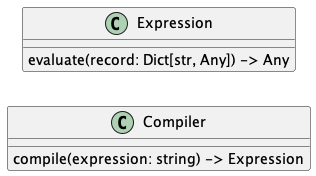
\includegraphics{diagrams/api_design-class.png}